\documentclass{article}

%% So you want a venn diagram in your proof? Awesome! I hear all the cool kids are using venn diagrams. Here's a basic template that you can modify to fit your needs.

%% In order to use tikz, you need to tell latex that you need the tikz package. If you're adding a venn diagram to an existing proof, make sure this line goes in the preamble.
\usepackage{tikz}


% Daniel discovered how to make Venn diagrams in Tex.  Below is his advice that we can all do this.

\begin{document}
\pagestyle{empty}

%% This block is what you'll need to put in your code where you want your picture.
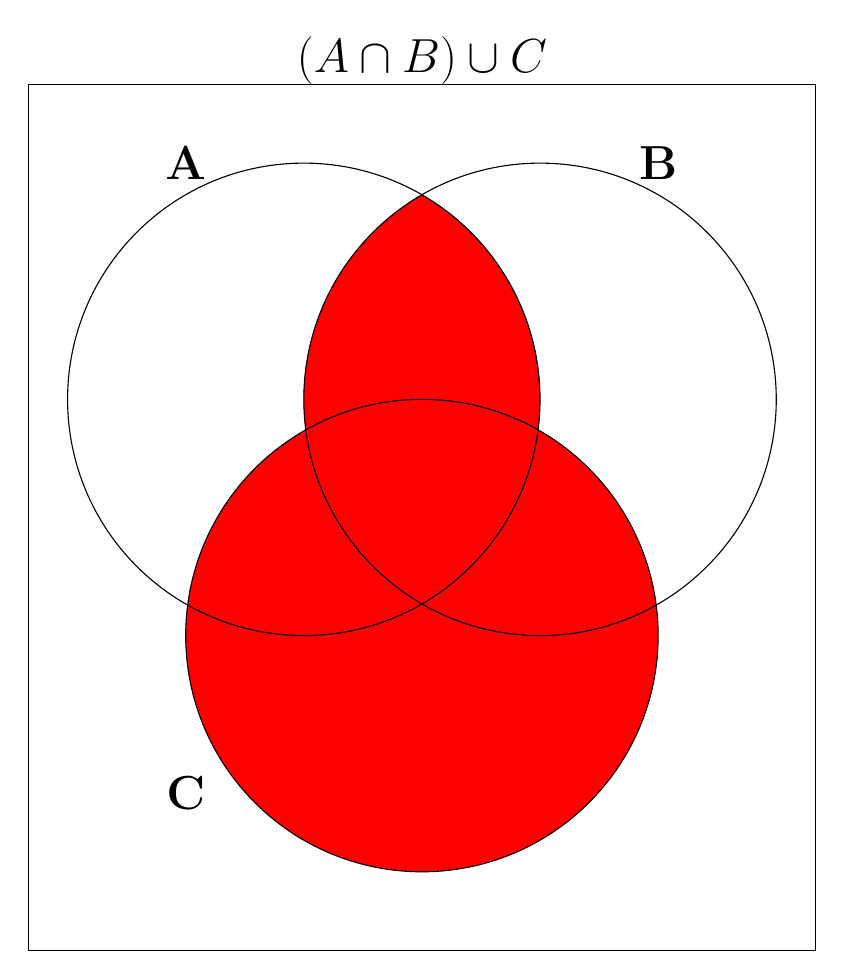
\begin{tikzpicture}
%% You can adjust the opacity here. For venn diagrams it is convenient to have a low opacity so that you can see intersections
	\begin{scope}
%% The draw command knows a lot of shapes. To make a rectangle you just need to specify two diagonal corners. Make sure you always have a semicolon at the end of your draw commands, otherwise latex flips out.
    \draw (-5,5) rectangle (5,-6);
    
%% Similarly, you can make a circle by specifying the center and then the radius. You can also add a fill color, but if you're printing in black and white you'll probably want to remove that line.
    \begin{scope}
    \clip (-1.5,1) circle (3);
    \clip (1.5,1) circle (3);
    \draw[fill=red, draw = black] (1.5,1) circle (3);
    \draw[fill=red, draw = black] (-1.5,1) circle (3);
    \end{scope}

    \draw[fill=red, draw = black] (0,-2) circle (3);
    \draw[draw = black] (1.5,1) circle (3);
    \draw[draw = black] (-1.5,1) circle (3);

    \node at (0,5.3) {\LARGE{$(A\cap B) \cup C$}};
    \node at (-3,4) {\LARGE\textbf{A}};
    \node at (3,4) {\LARGE\textbf{B}};
    \node at (-3,-4) {\LARGE\textbf{C}};
    \end{scope}

\end{tikzpicture}

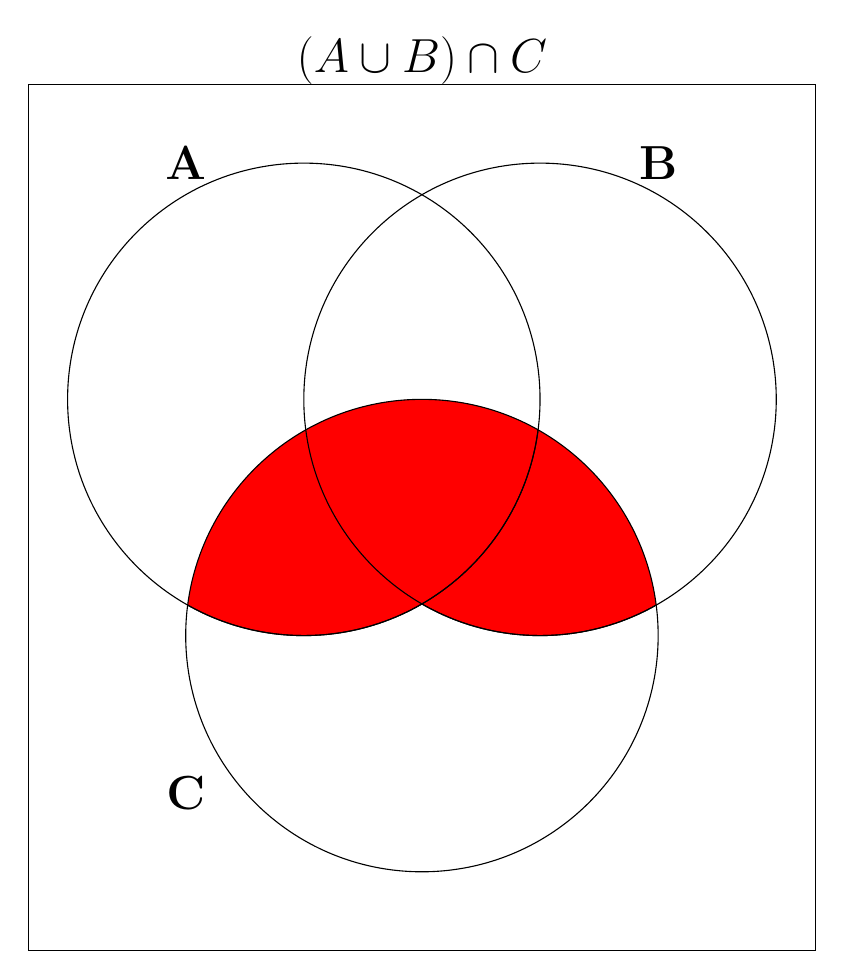
\begin{tikzpicture}
    %% You can adjust the opacity here. For venn diagrams it is convenient to have a low opacity so that you can see intersections
        \begin{scope}
    %% The draw command knows a lot of shapes. To make a rectangle you just need to specify two diagonal corners. Make sure you always have a semicolon at the end of your draw commands, otherwise latex flips out.
        \draw (-5,5) rectangle (5,-6);
        
    %% Similarly, you can make a circle by specifying the center and then the radius. You can also add a fill color, but if you're printing in black and white you'll probably want to remove that line.
    \begin{scope}
        \clip (0,-2) circle (3);
        \draw[fill=red, draw = black] (1.5,1) circle (3);
        \draw[fill=red, draw = black] (-1.5,1) circle (3);
    \end{scope}
    \begin{scope}
        \draw[draw = black] (1.5,1) circle (3);
        \draw[draw = black] (-1.5,1) circle (3);
        \draw[draw = black] (0,-2) circle (3);
    \end{scope}
        \node at (0,5.3) {\LARGE{$(A\cup B) \cap C$}};
        \node at (-3,4) {\LARGE\textbf{A}};
        \node at (3,4) {\LARGE\textbf{B}};
        \node at (-3,-4) {\LARGE\textbf{C}};
        \end{scope}
    
    \end{tikzpicture}
    
\end{document}